% Created 2020-04-04 Sat 18:42
% Intended LaTeX compiler: pdflatex
\documentclass[11pt]{article}
\usepackage[utf8x]{inputenc}
\usepackage[T1]{fontenc}
\usepackage{graphicx}
\usepackage{grffile}
\usepackage{longtable}
\usepackage{wrapfig}
\usepackage{rotating}
\usepackage[normalem]{ulem}
\usepackage{amsmath}
\usepackage{textcomp}
\usepackage{amssymb}
\usepackage{capt-of}
\usepackage{hyperref}
\usepackage{unicode-math}
\author{Gianluca Scarpellini (gianluca@scarpellini.dev)}
\date{\today}
\title{Project 1 - Deep reinforcement learning - Navigation}
\hypersetup{
 pdfauthor={Gianluca Scarpellini (gianluca@scarpellini.dev)},
 pdftitle={Project 1 - Deep reinforcement learning - Navigation},
 pdfkeywords={},
 pdfsubject={},
 pdfcreator={Emacs 26.3 (Org mode 9.3.6)}, 
 pdflang={English}}
\begin{document}

\maketitle
\tableofcontents


\section{Introduction}
\label{sec:org28be15a}
Deep Reinforcement Learning is today becoming a relevant field of research. The
current work aims to evaluate the ability of value-based methods of solving a
simple task in a constrained environment. In particular, we implemented Deep
Q-learning algorithm as presented during Udacity "Deep Reinforcement Learning"
as well as in the original paper. We describe the environment in section
\ref{sec:org7be0c40}. A more in depth explanation of Deep Q-learning is presented in
section \ref{sec:org84462b5}. In section \ref{sec:org551cb12} we comment the results
obtained with the algorithm. Finally, we take our conclusions in section \ref{sec:org5f8d235}


\section{Environment and task}
\label{sec:org7be0c40}
The presented project is developed in order to solve the "Banana"
environment. The task consists in collecting yellow banana in a plain space
while avoiding blue banana. The agent needs to learn the optimal policy. It gets
a reward of +1 for each yellow banana and a reward of -1 for each blue
banana. The action space is limited to 4 possible choices: move left, right,
forward and backward. 

\section{Algorithm and Implementation}
\label{sec:org84462b5}
We decided to solve the environment with Deep Q-learning algorithm. Deep
Q-Learning has already shown its potential in solving Atari games as well (or
better then) human players. It's an off-policy learning algorithm. 2 different
policies are kept simultaneously: an evaluation policy and the learned
policy. Q-learning, and temporal-difference learning algorithms in general,
learn an action-value function Q from each step of each episode. Compared to
Monte-carlo methods, TD-methods reduces learning time at the cost of an
additional \textbf{bias}. The equation in figure \ref{fig:org2050936} refers to the vanilla
pnpQ-Learning update. Q function is updated using a \textbf{future} value estimation
(which introduces bias in the learning process). Modern development of Deep
Learning and Neural Networks can be exploited for \textbf{approximating} function Q
with function approximators. 

\begin{figure}[htbp]
\centering
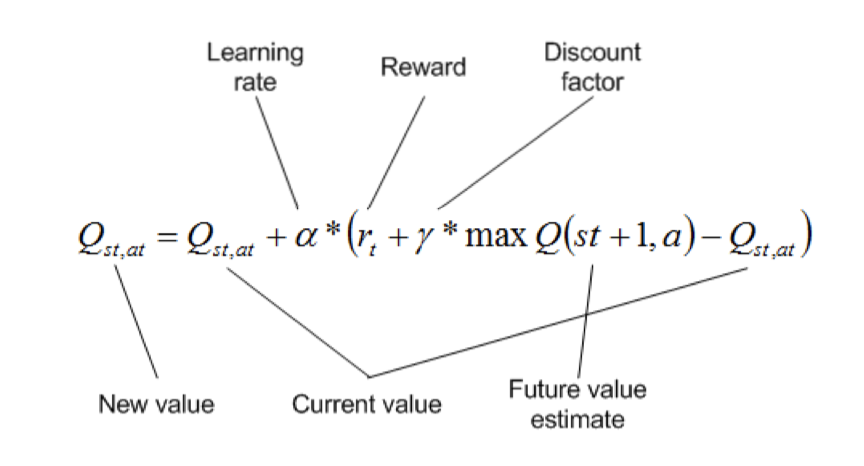
\includegraphics[width=.9\linewidth]{./contents/equation.png}
\caption{\label{fig:org2050936}Q-Learning equation}
\end{figure}

The main idea of Deep Q-Learning is contained in figure \ref{fig:org0663b55}. In particular,
Deep Q-learning implements 2 techniques in order to stabilize the training
process and allow the neural network to learn the \textbf{optimal} action-value
function.
\begin{itemize}
\item Fixed Q-target: 2 different networks are combined in order to keep the method
\end{itemize}
off-policy. A target network is updated at every iteration while an evaluation
network is exploited for future value estimation. The target network parameters
are copied to the evaluation network at the end of the updating phase.

\begin{itemize}
\item Experience Replay: In order to decouple sequential states of each episode,
\end{itemize}
Deep Q-Learning create a buffer of tuple <S, a, R, S'>. At each iteration a
random batch is pulled from the buffer. The main goal of experience replay is to
feed into the learning algorithm independents batch of tuples.

\begin{figure}[htbp]
\centering
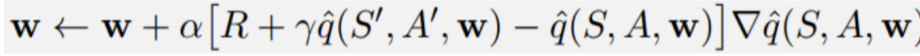
\includegraphics[width=.9\linewidth]{./contents/dql.png}
\caption{\label{fig:org0663b55}Deep Q-Learning equation weights update equation}
\end{figure}

\subsection{Hyperparameters}
\label{sec:orge1e8cf0}
For the experiment we used the following hyperparameters:

\begin{center}
\begin{tabular}{lr}
Hyperpameter & Value\\
\hline
lr & 5e-4\\
tau & 1e-3\\
gamma & 0.99\\
update every & 4\\
buffer size & 1e5\\
n. hidden layers & 2\\
\hline
\end{tabular}
\end{center}


\section{Results}
\label{sec:org551cb12}
In figure \ref{fig:orgf52b795} it's presented the algorithm result per episode. In
particular, we were able to solve the environment in less then 300 epochs. The
scores kept growing until an optimal maximum of 13, probably due to limited time
play per episode. The learning phase was revealed to be a noisy. More stables
approaches are discussed in section \ref{sec:org5f8d235}. 

\begin{figure}[htbp]
\centering
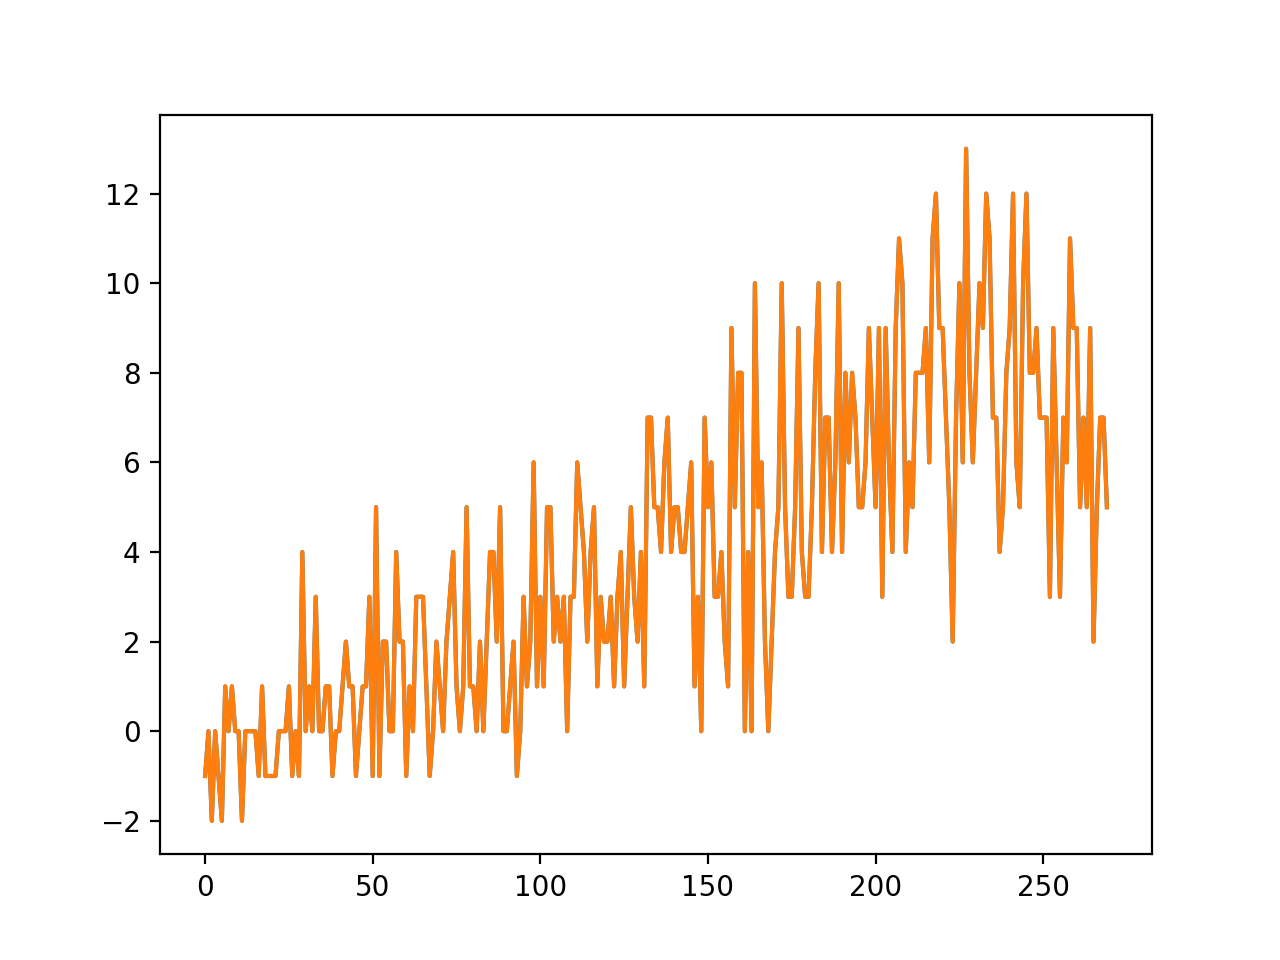
\includegraphics[width=.9\linewidth]{./contents/agent.png}
\caption{\label{fig:orgf52b795}Learning scores per epoch}
\end{figure}

\section{Conclusion and further}
\label{sec:org5f8d235}
We developed a pipeline in order to solve `banana` environment with Deep
Reinforcement Learning. In particular, we implemented \textbf{Deep Q-Learning}
following the paper specification. Deep Q-learning is an off-policy algorithm
which has proven stability and optimal results in multiple tasks. We got the
algorithm to hack the environment in less then 300 epochs. As discussed above,
we believe the noisy of the learning could be alleviated with further
developments of both learning phase and the buffering phase. We would consider
integrating \textbf{Prioritized Replay} as a way to optimally sample mini-batches from
the queue. Further improvements are available in implementing \textbf{Double DQNs}
strategy in order to disentangle the calculation of Q-targets for best action
estimation from Q-values.
\end{document}